\documentclass[ignorenonframetext,aspectratio=169]{beamer}
\setbeamertemplate{caption}[numbered]
\setbeamertemplate{caption label separator}{: }
\setbeamercolor{caption name}{fg=normal text.fg}
\beamertemplatenavigationsymbolsempty
\usepackage{lmodern}
\usepackage{amssymb,amsmath}
\usepackage{ifxetex,ifluatex}
\usepackage{fixltx2e} % provides \textsubscript
\ifnum 0\ifxetex 1\fi\ifluatex 1\fi=0 % if pdftex
  \usepackage[T1]{fontenc}
  \usepackage[utf8]{inputenc}
\else % if luatex or xelatex
  \ifxetex
    \usepackage{mathspec}
  \else
    \usepackage{fontspec}
  \fi
  \defaultfontfeatures{Ligatures=TeX,Scale=MatchLowercase}
\fi
% use upquote if available, for straight quotes in verbatim environments
\IfFileExists{upquote.sty}{\usepackage{upquote}}{}
% use microtype if available
\IfFileExists{microtype.sty}{%
\usepackage{microtype}
\UseMicrotypeSet[protrusion]{basicmath} % disable protrusion for tt fonts
}{}
\newif\ifbibliography
\hypersetup{
            pdftitle={Welcome to 142: Introduction to Probability and Statistics in Biology and Public Health},
            pdfborder={0 0 0},
            breaklinks=true}
\urlstyle{same}  % don't use monospace font for urls
\usepackage{longtable,booktabs}
\usepackage{caption}
% These lines are needed to make table captions work with longtable:
\makeatletter
\def\fnum@table{\tablename~\thetable}
\makeatother
\usepackage{graphicx,grffile}
\makeatletter
\def\maxwidth{\ifdim\Gin@nat@width>\linewidth\linewidth\else\Gin@nat@width\fi}
\def\maxheight{\ifdim\Gin@nat@height>\textheight0.8\textheight\else\Gin@nat@height\fi}
\makeatother
% Scale images if necessary, so that they will not overflow the page
% margins by default, and it is still possible to overwrite the defaults
% using explicit options in \includegraphics[width, height, ...]{}
\setkeys{Gin}{width=\maxwidth,height=\maxheight,keepaspectratio}

% Prevent slide breaks in the middle of a paragraph:
\widowpenalties 1 10000
\raggedbottom

\AtBeginPart{
  \let\insertpartnumber\relax
  \let\partname\relax
  \frame{\partpage}
}
\AtBeginSection{
  \ifbibliography
  \else
    \let\insertsectionnumber\relax
    \let\sectionname\relax
    \frame{\sectionpage}
  \fi
}
\AtBeginSubsection{
  \let\insertsubsectionnumber\relax
  \let\subsectionname\relax
  \frame{\subsectionpage}
}

\setlength{\parindent}{0pt}
\setlength{\parskip}{6pt plus 2pt minus 1pt}
\setlength{\emergencystretch}{3em}  % prevent overfull lines
\providecommand{\tightlist}{%
  \setlength{\itemsep}{0pt}\setlength{\parskip}{0pt}}
\setcounter{secnumdepth}{0}
\usetheme{Goettingen}
\renewcommand{\textbf}{\structure}
\renewcommand{\mathbf}{\structure}
\addtobeamertemplate{navigation symbols}{}{ \usebeamerfont{footline} }
\addtobeamertemplate{navigation symbols}{}{ \usebeamercolor[fg]{footline} }
\addtobeamertemplate{navigation symbols}{}{ \insertframenumber/\inserttotalframenumber }
\usepackage[os=win]{menukeys}
\usepackage{soul}
\usepackage{xcolor}
\usepackage{caption}
\usepackage[os=win]{menukeys}
\usepackage{copyrightbox}

\title{Welcome to 142: Introduction to Probability and Statistics in Biology
and Public Health}
\date{January 22 2020}

\begin{document}
\frame{\titlepage}

\begin{frame}

\end{frame}

\subsection{What is this class?}\label{what-is-this-class}

\begin{frame}{What is this class?}

\begin{figure}
\centering
\includegraphics{word_cloud.png}
\caption{What do you think of when you think about statistics?}
\end{figure}

\end{frame}

\begin{frame}{What is this class?}

In this class we are going to think about

\begin{itemize}
\item
  \textbf{DATA} - How we gather, display and summarize information
\item
  \textbf{Probability } - the role of chance
\item
  \textbf{Statistics} - the science of drawing statistical conclusions
  from data using a knowledge of probability
\end{itemize}

\end{frame}

\begin{frame}{Three parts}

\begin{itemize}
\tightlist
\item
  Part I: learning to explore and summarize univariate and bivariate
  distributions.
\item
  Part II: classical problems in probability and the some commonly used
  probability distributions and the central limit theorem
\item
  Part III: statistical inference, the process of estimating statistics
  from samples to make inference about populations
\end{itemize}

\end{frame}

\begin{frame}{Goals for the semester}

In addition the the learning objectives listed in your syllabus our
overarching goals for the semester are to develop:

\begin{itemize}
\tightlist
\item
  your ability to critically assess statistical information presented to
  you in scientific and non-scientific fora
\item
  your sense of how to approach answering real world questions with data
\item
  your ability to concisely and accurately describe statistical methods
  and results
\end{itemize}

\end{frame}

\begin{frame}{This is not a math class}

Statistics is often classified as a branch of math, but I'd argue that
it is more important to \textbf{focus on the connections that statistics
has with science} (how we can learn about the world through data)

Though it is true that statistics uses math (and sometimes fairly
advanced math!), \textbf{not much math is needed} to learn introductory
statistics

In this class we will try, as much as possible, to \textbf{emphasize
concepts} and help you develop your statistical intuition

\end{frame}

\begin{frame}{This is not a programming class}

Statistics is often viewed as ``just computer programming,'' but this is
an incorrect and dangerous characterization: \textbf{computer
programming is simply a tool for conducting statistical analysis}

The use of computer programming in statistics is---and should
be---\textbf{quite different} than approaches to non-statistical
programming

We are using r programming in this course because it is an extremely
useful skill, facilitates computation, and is desired in the job market

\end{frame}

\begin{frame}{This is a relevant class}

I hope to convince everyone here that statistics is relevant to everyone

You make many decisions during your day that are influenced by
statistics

Statistics is not just relevant for \textbf{public health}, but also for
other professions, including: policy, journalism and law

As we'll try to illustrate via the recurring ``statistics is
everywhere'' segments, \textbf{statistics is useful for understanding
the news} and the world around us

\end{frame}

\subsection{Course logistics}\label{course-logistics}

\begin{frame}{Teaching Team}

Instructor

Mi-Suk Kang Dufour, PhD, MPH

GSIs (short bios are on bcourses) Asem Berkalieva, Aidean McLoughlin,
Sophia (Sophie) Fuller, Yi Li, Dorothy Chen, and Hao Wang.

Course tutors: Cam Adams, Simran Bajwa

Technical wizard: Nolan Pokpongkiat

\end{frame}

\begin{frame}{Structure}

Lecture: Introduction of concepts

Lab: Practice with programming

Discussion: Review of key concepts, application of knowledge to reading
and writing in scientific litterature

\end{frame}

\begin{frame}{Waitlist status and Section shifting}

As of today it looks like almost all wait-listed students should be able
to enroll

We expect some shifting for the first few weeks.

Attend your enrolled section

\end{frame}

\begin{frame}{Accomodations}

Make requests in writing by February 1st so that any accommodations can
be implemented in time for the first midterm exam

If your DSP accomodation allows extension on take home assignments we
ask that you discuss your request no later than 24 hours after the
assignment is posted.

If you need an accomodation but do not yet have an official letter apply
as soon as possible:
\url{https://dsp.berkeley.edu/students/new-students}.

\end{frame}

\begin{frame}{Communication}

\textbf{Please please please ask questions!!!}

Questions during lecture, discussion and lab section are strongly
encouraged. If something is unclear to you, it is probably unclear to
many others in the room.

\textbf{Use the discussion board}

We will use piazza for class announcements and discussion.

\textbf{Email} only for logistical or non-content related issues

\end{frame}

\begin{frame}{Office hours}

GSIs will hold office hours every week - office hours will be posted on
the website

Instructor office hours will be limited and by appointment only

\end{frame}

\begin{frame}{Grading}

Course grades are based on the following activities:

\begin{itemize}
\tightlist
\item
  In Class participation and quizzes 10\%
\item
  Lab participation 5\%
\item
  Problem sets: 20\%
\item
  Optional Extra credit: up to 2 points on total grade
\item
  Midterm Exam 1: 15\%
\item
  Midterm Exam 2: 15\%
\item
  Data project: 10\%
\item
  Final Exam: 25\%
\end{itemize}

\end{frame}

\begin{frame}{Grading process}

\begin{itemize}
\tightlist
\item
  Gradescope
\item
  Blinded
\item
  Student peer reviews
\end{itemize}

\end{frame}

\begin{frame}{Grades}

\begin{figure}
\centering
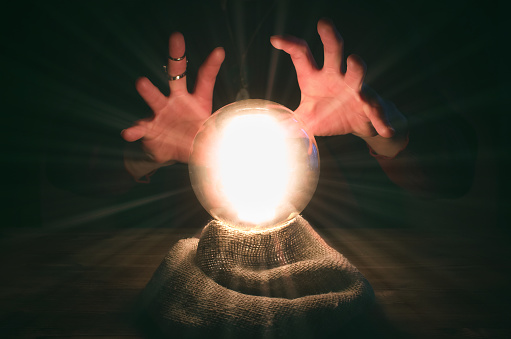
\includegraphics{crystalball.jpg}
\caption{Will I get an A?}
\end{figure}

\end{frame}

\subsection{Ongoing evolution of the
course}\label{ongoing-evolution-of-the-course}

\subsection{Participation}\label{participation}

\subsection{Statistics is Everywhere}\label{statistics-is-everywhere}

\begin{frame}{Warning labels for coffee in California?}

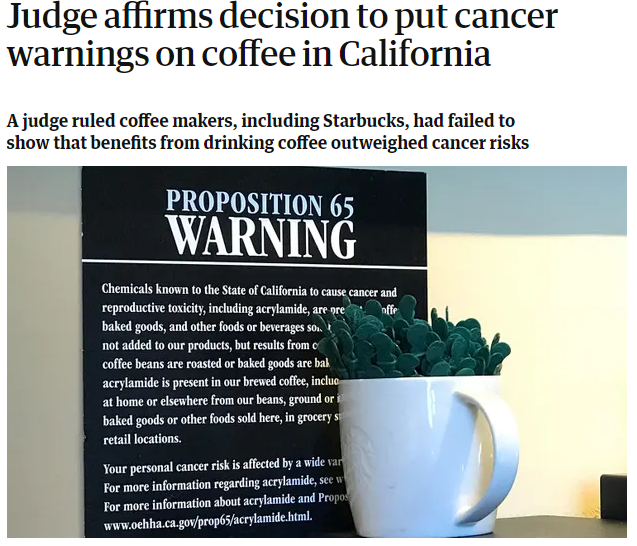
\includegraphics{warning.png} \textbf{Warning regarding acrylamide} at a
Starbucks location in Burbank, California.

\end{frame}

\begin{frame}{Warning labels for coffee in California?}

\begin{itemize}
\tightlist
\item
  from
  \emph{\href{https://www.nytimes.com/2018/04/23/upshot/california-coffee-and-cancer-one-of-these-doesnt-belong.html}{\textcolor[HTML]{ffa328}{\ul{The New York Times}}}},
  April 2018:
\end{itemize}

\begin{quote}
\textbf{California's Proposition 65, enacted in 1986, mandates that
businesses with more than 10 employees warn consumers if their products
contain one of many chemicals that the state has ruled as carcinogenic.}
\end{quote}

\begin{itemize}
\tightlist
\item
  and:
\end{itemize}

\begin{quote}
One of these chemicals is \textbf{acrylamide}.
\end{quote}

\end{frame}

\begin{frame}{Warning labels for coffee in California?}

\begin{itemize}
\tightlist
\item
  from
  \emph{\href{http://www.latimes.com/local/lanow/la-me-coffee-tabels-20180329-story.html}{\textcolor[HTML]{ffa328}{\ul{The Los Angeles Times}}}},
  March 2018:
\end{itemize}

\begin{quote}
\textbf{Acrylamide is created when coffee is roasted} and also is found
in fried potatoes and burnt toast. It has been found to increase cancer
risk in rodents. \textbf{Its effect on humans remains inconclusive.}
\end{quote}

\end{frame}

\begin{frame}{Warning labels for coffee in California?}

\begin{itemize}
\tightlist
\item
  more from the \emph{New York Times} article:
\end{itemize}

\begin{quote}
\textbf{we have a wealth of evidence about coffee's effects}. Meta
analyses have shown that coffee is associated with lower risks of liver
cancer, and no increased risk of prostate cancer or breast cancer. When
we look at cancer over all, it appears that \textbf{coffee---if
anything---is associated with a lower risk of cancer}.
\end{quote}

\end{frame}

\begin{frame}{Warning labels for coffee in California?}

\begin{itemize}
\tightlist
\item
  even more from the \emph{New York Times} article:
\end{itemize}

\begin{quote}
The more serious problem with California's law is one of effect size.
\textbf{Consumers can't just be concerned with whether a danger exists;
they also need to be concerned about the magnitude of that risk.} Even
if there's a statistically significant risk between huge quantities of
coffee and some cancer (and that's not proven), it's very, very small.
\end{quote}

\end{frame}

\begin{frame}{Warning labels for coffee in California?}

The scientific studies mentioned in these articles relied heavily on
\textbf{statistics} This example contains several concepts we will cover
in this class including:

\begin{itemize}
\tightlist
\item
  The importance of where the data come from (sampling and target
  population)
\item
  Mechanism for exposure assignment (random vs non-random)
\item
  The importance of how much data are available (sample size)
\item
  The quality of the data (measurement error)
\item
  The concept of statistical association vs causal association
\item
  The difference between statistical significance and clinical
  significance
\end{itemize}

\end{frame}

\begin{frame}{Warning labels for coffee in California?}

The international concensus\ldots{}

\href{https://www.thelancet.com/journals/lanonc/article/PIIS1470-2045(16)30239-X/fulltext}{\textcolor[HTML]{ffa328}{\ul{International Agency for Research on Cancer (IARC)}}}:

\begin{quote}
coffee is \emph{unclassifiable} with respect to carcinogenicity in
humans
\end{quote}

And more recently in California\ldots{}

\href{https://www.npr.org/2018/08/30/643246149/coffee-does-not-merit-cancer-warning-label-ordered-in-california-fda-says}{\textcolor[HTML]{ffa328}{\ul{from NPR}}}:

\begin{quote}
FDA Commissioner Scott Gottlieb said in a statement that ``if a state
law purports to require food labeling to include a false or misleading
statement, the FDA may decide to step in.''
\end{quote}

\begin{quote}
He added that \textbf{a large body of research has found little evidence
that coffee causes cancer}
\end{quote}

\begin{quote}
New regulation took effect Oct 1 2019 ``Exposures to chemicals in
coffee, listed on or before March 15, 2019, as known to the state to
cause cancer, that are created by and inherent in the processes of
roasting coffee beans or brewing coffee, do not pose a significant risk
of cancer.''
\end{quote}

\end{frame}

\begin{frame}{Warning labels for coffee in California?}

As public health practitioners we are concerned with what happens to the
public perception of science when these kinds of warnings are issued

We should aim to be better at communicating our findings to inform
policy and public opinion.

\end{frame}

\begin{frame}{Consequences of poor communication}

\begin{figure}
\centering
\includegraphics{LWT_science.png}
\caption{\url{https://www.statnews.com/2016/05/09/john-oliver-bad-science/}}
\end{figure}

\end{frame}

\subsection{PPDAC - the approach we will use to answering questions with
statistics}\label{ppdac---the-approach-we-will-use-to-answering-questions-with-statistics}

\begin{frame}{Problem}

A clear statement of what we are trying to achieve.

\end{frame}

\begin{frame}{Three main problem types}

\begin{itemize}
\tightlist
\item
  \textbf{Descriptive}: learning about some particular attribute of a
  population
\item
  \textbf{Causative/Etiologic}: do changes in an explanatory variable
  cause changes in a response variable?
\item
  \textbf{Predictive}: how can we best predict the value of the response
  variable for an individual?
\end{itemize}

\end{frame}

\begin{frame}{Problem type?}

\begin{itemize}
\item
  Insurance company: What is the probability (how likely is it) that a
  25 year old unmarried male driver has a car accident?
\item
  Health department: How many cases of influenza have we seen this
  season compared to last season?
\item
  Health care system: If we treat patients with diabetes using
  medication X, will thier insulin regulation be better or worse than
  medication y?
\end{itemize}

\end{frame}

\begin{frame}{Plan}

The procedures we use to carry out the study.

\begin{itemize}
\tightlist
\item
  \textbf{Census} or \textbf{sample} from the target population?

  \begin{itemize}
  \tightlist
  \item
    How was the sampling conducted?
  \item
    Was the sample random?
  \end{itemize}
\item
  Is the study prospective or retrospective?
\item
  Is the study observational or experimental?
\end{itemize}

\end{frame}

\begin{frame}{Data}

The data which is collected according to the Plan.

\begin{itemize}
\tightlist
\item
  How many observations to we have?
\item
  How relaible are the measures?
\end{itemize}

\end{frame}

\begin{frame}{Analysis}

The data is summarized and analysed to answer the questions posed by the
Problem.

We use our knowledge about probabilities to assess the role of chance in
our findings.

\end{frame}

\begin{frame}{Conclusion}

Conclusions are drawn about what has been learned about answering the
Problem.

\end{frame}

\subsection{PPDAC Example 1: A smoking behaviour
study}\label{ppdac-example-1-a-smoking-behaviour-study}

\begin{frame}{PPDAC Example}

Problem: Suppose we wish to study the smoking behavior of California
residents aged 14-20 years.

In particular, we are interested in the \emph{prevalence} of current
smoking by gender.

What type of problem is this?

\end{frame}

\begin{frame}{PPDAC Example}

Plan: We need to first choose a time period, because we know that
smoking behavior has changed immensely over time. It is unfeasible to
gather these data for all residents in California who are 14-20 years
old.

Instead we conduct a \emph{random sample} of size \(n\) persons. We
collect their: age, gender, and smoking status.

Note that we need to decide how large \(n\) should be, and how to obtain
the random sample. The latter question is, in particular, very important
if we want to ensure that our sample is representative of the population
of interest. Time and money also constrain how the sample will be
collected.

\end{frame}

\begin{frame}{PPDAC Example}

Data: Suppose that a random sample of 200 persons aged 14-20 was
selected, yielding these data:

\begin{longtable}[]{@{}llll@{}}
\toprule
Gender & Number of smokers & Number of non-smokers &
Total\tabularnewline
\midrule
\endhead
Teen girls and women & 32 & 66 & 98\tabularnewline
Teen boys and men & 27 & 75 & 102\tabularnewline
Total & 59 & 141 & 200\tabularnewline
\bottomrule
\end{longtable}

\end{frame}

\begin{frame}{PPDAC Example}

Analysis: The proportion of women in the sample who smoke is 32/98 =
33\%. The proportion of men in the sample who smoke is 27/102 = 26\%.

We would also like some idea as to how close this estimate is likely to
be from the actual proportion in the population.

If we selected a second random sample of the same size, we would likely
estimate different proportions for men and women. We will learn how to
estimate the precision of these estimates.

\end{frame}

\begin{frame}{PPDAC Example}

Conclusion: 33\% of girls and women aged 14-20 and 26\% of boys and men
of the same age group are current smokers in California in 2018 (plus a
measure of uncertainty).

\end{frame}

\subsection{Example 2: Life expectancy for non-Hispanic black and white
men and women in California between
1969-2013}\label{example-2-life-expectancy-for-non-hispanic-black-and-white-men-and-women-in-california-between-1969-2013}

\begin{frame}{Introduction}

Life expectancy is one of the core measures used in public health to
comment on the well-being of groups of people. Differences in life
expectancy by race/ethnicity, for individuals living in the same region
can reflect underlying inequalities in policies, access to care, food
environments, structural and systemic racism, among other potential
causes.

\end{frame}

\begin{frame}{Research objective (Problem)}

The purpose of this short report is to visualize life expectancy among
black and white men and women in California between 1969 and 2013.

We are interested in whether there are differences by group and whether
these differences have changed over time.

What type of problem is this?

\end{frame}

\begin{frame}{Plan}

Death certificates in the United States include race/ethnicity, age at
death, and date of death and capture all deaths of US residents. These
data are aggregated by the
\href{https://seer.cancer.gov/seerstat/}{CDC's National Cancer
Institute} into the SEER*Stat software. Previously, Riddell et
al.\textsuperscript{1}, analyzed these data to compute estimated trends
in life expectancy for non-Hispanic black and white men and women, for
40 US states between 1969 and 2013. States without enough data were
excluded from these analyses.

To carry out this short report, we will use data from Riddell et al. to
visualize trends in life expectancy as part of an exploratory data
analysis. In particular, we will plot time trends for black and white
men and women in California.

\end{frame}

\begin{frame}{Data}

Here are the first few rows of these data for California:

\begin{figure}
\centering
\includegraphics{ca_le.png}
\caption{}
\end{figure}

\end{frame}

\begin{frame}{Analysis}

\includegraphics{lec01-intro_files/figure-beamer/first-look-time-plots-1.pdf}

\end{frame}

\begin{frame}{Analysis}

\includegraphics{lec01-intro_files/figure-beamer/reshape-and-compute-LE-difference-1.pdf}

\end{frame}

\begin{frame}{Conclusion}

The difference in life expectancy in 1969 between non-Hispanic blacks
and whites was 5.1 years for men and 4.5 for women in California.

By 2013, the difference was 4.3 years for men and 3.6 for women in
California.

\end{frame}

\begin{frame}{References}

The PPDAC method is described based on course notes from STAT 231 from
the University of Waterloo (Ontario, Canada). Spring 2006 Course Packet.

\begin{enumerate}
\def\labelenumi{\arabic{enumi}.}
\tightlist
\item
  Riddell CA, Morrison KT, Harper S, Kaufman JS. Trends in the
  contribution of major causes of death to the black-white life
  expectancy gap by US state. \textbf{Health \& Place}. 2018. 52:85-100.
  doi: 10.1016/j.healthplace.2018.04.003.
\end{enumerate}

\end{frame}

\begin{frame}{Parting Humor}

\begin{figure}
\centering
\includegraphics{science_news_cycle.png}
\caption{From PHDcomics.com}
\end{figure}

\end{frame}

\end{document}
